\subsection{Assurance Argument}

The assurance argument for the run-time assurance architecture is made explicit using Resolute~\cite{resolute}.  Resolute is a tool for specifying and instantiating assurance patterns, and analyzing the resulting assurance argument to determine whether all claims are supported by evidence.  Resolute is a plugin for the Open Source AADL Tool Environment (OSATE), which provides tight coupling between an assurance argument and the system architecture under evaluation.  Consequently, Resolute is able to instantiate the assurance pattern with context specified within the system model, extract evidence for supporting assurance claims, and produce a ``passing'' or ``failing'' assurance argument based on whether all claims are satisfied.

Figure~\ref{fig:rta-resolute} depicts the assurance argument for the run-time assurance architecture.  The full argument is not shown due to space constraints, but the general structure consists of a top-level claim supported by three sub-claims.  Overall, we wish to argue that the RTA architecture ensures that a safe flight plan is published (claim G1 in the figure).  In the event that the flight plan produced by the LEC is not deemed safe, we fall back on the backup flight plan produced by the BAF.  We therefore include the assumption (A1) that the BAF flight plan is indeed safe.

We argue the top-level goal is achieved by providing evidence that the architecture is correct (G4), the implementation logic is correct (G3), and that an unsafe flight plan can be detected when it is produced by the LEC (G2).  The architecture correctness argument is comprised of multiple sub-claims that focus on correct model composition with respect to requirements.  As shown in the figure, one method for demonstrating correctness is AGREE verification (G14).  This particular branch of the assurance argument also demonstrates Resolute's ability to evaluate evidence produced by external tools as part of evaluating the assurance argument.
%
The implementation logic correctness argument includes is supported by a proof of correctness from the APT tool (G9). The safe backup sub-claim argues that the decision from run-time monitor is safe. The evidence for this claim ensures that both the run-time monitor requirements and implementation is correct. 

\begin{figure*}
	\centering
	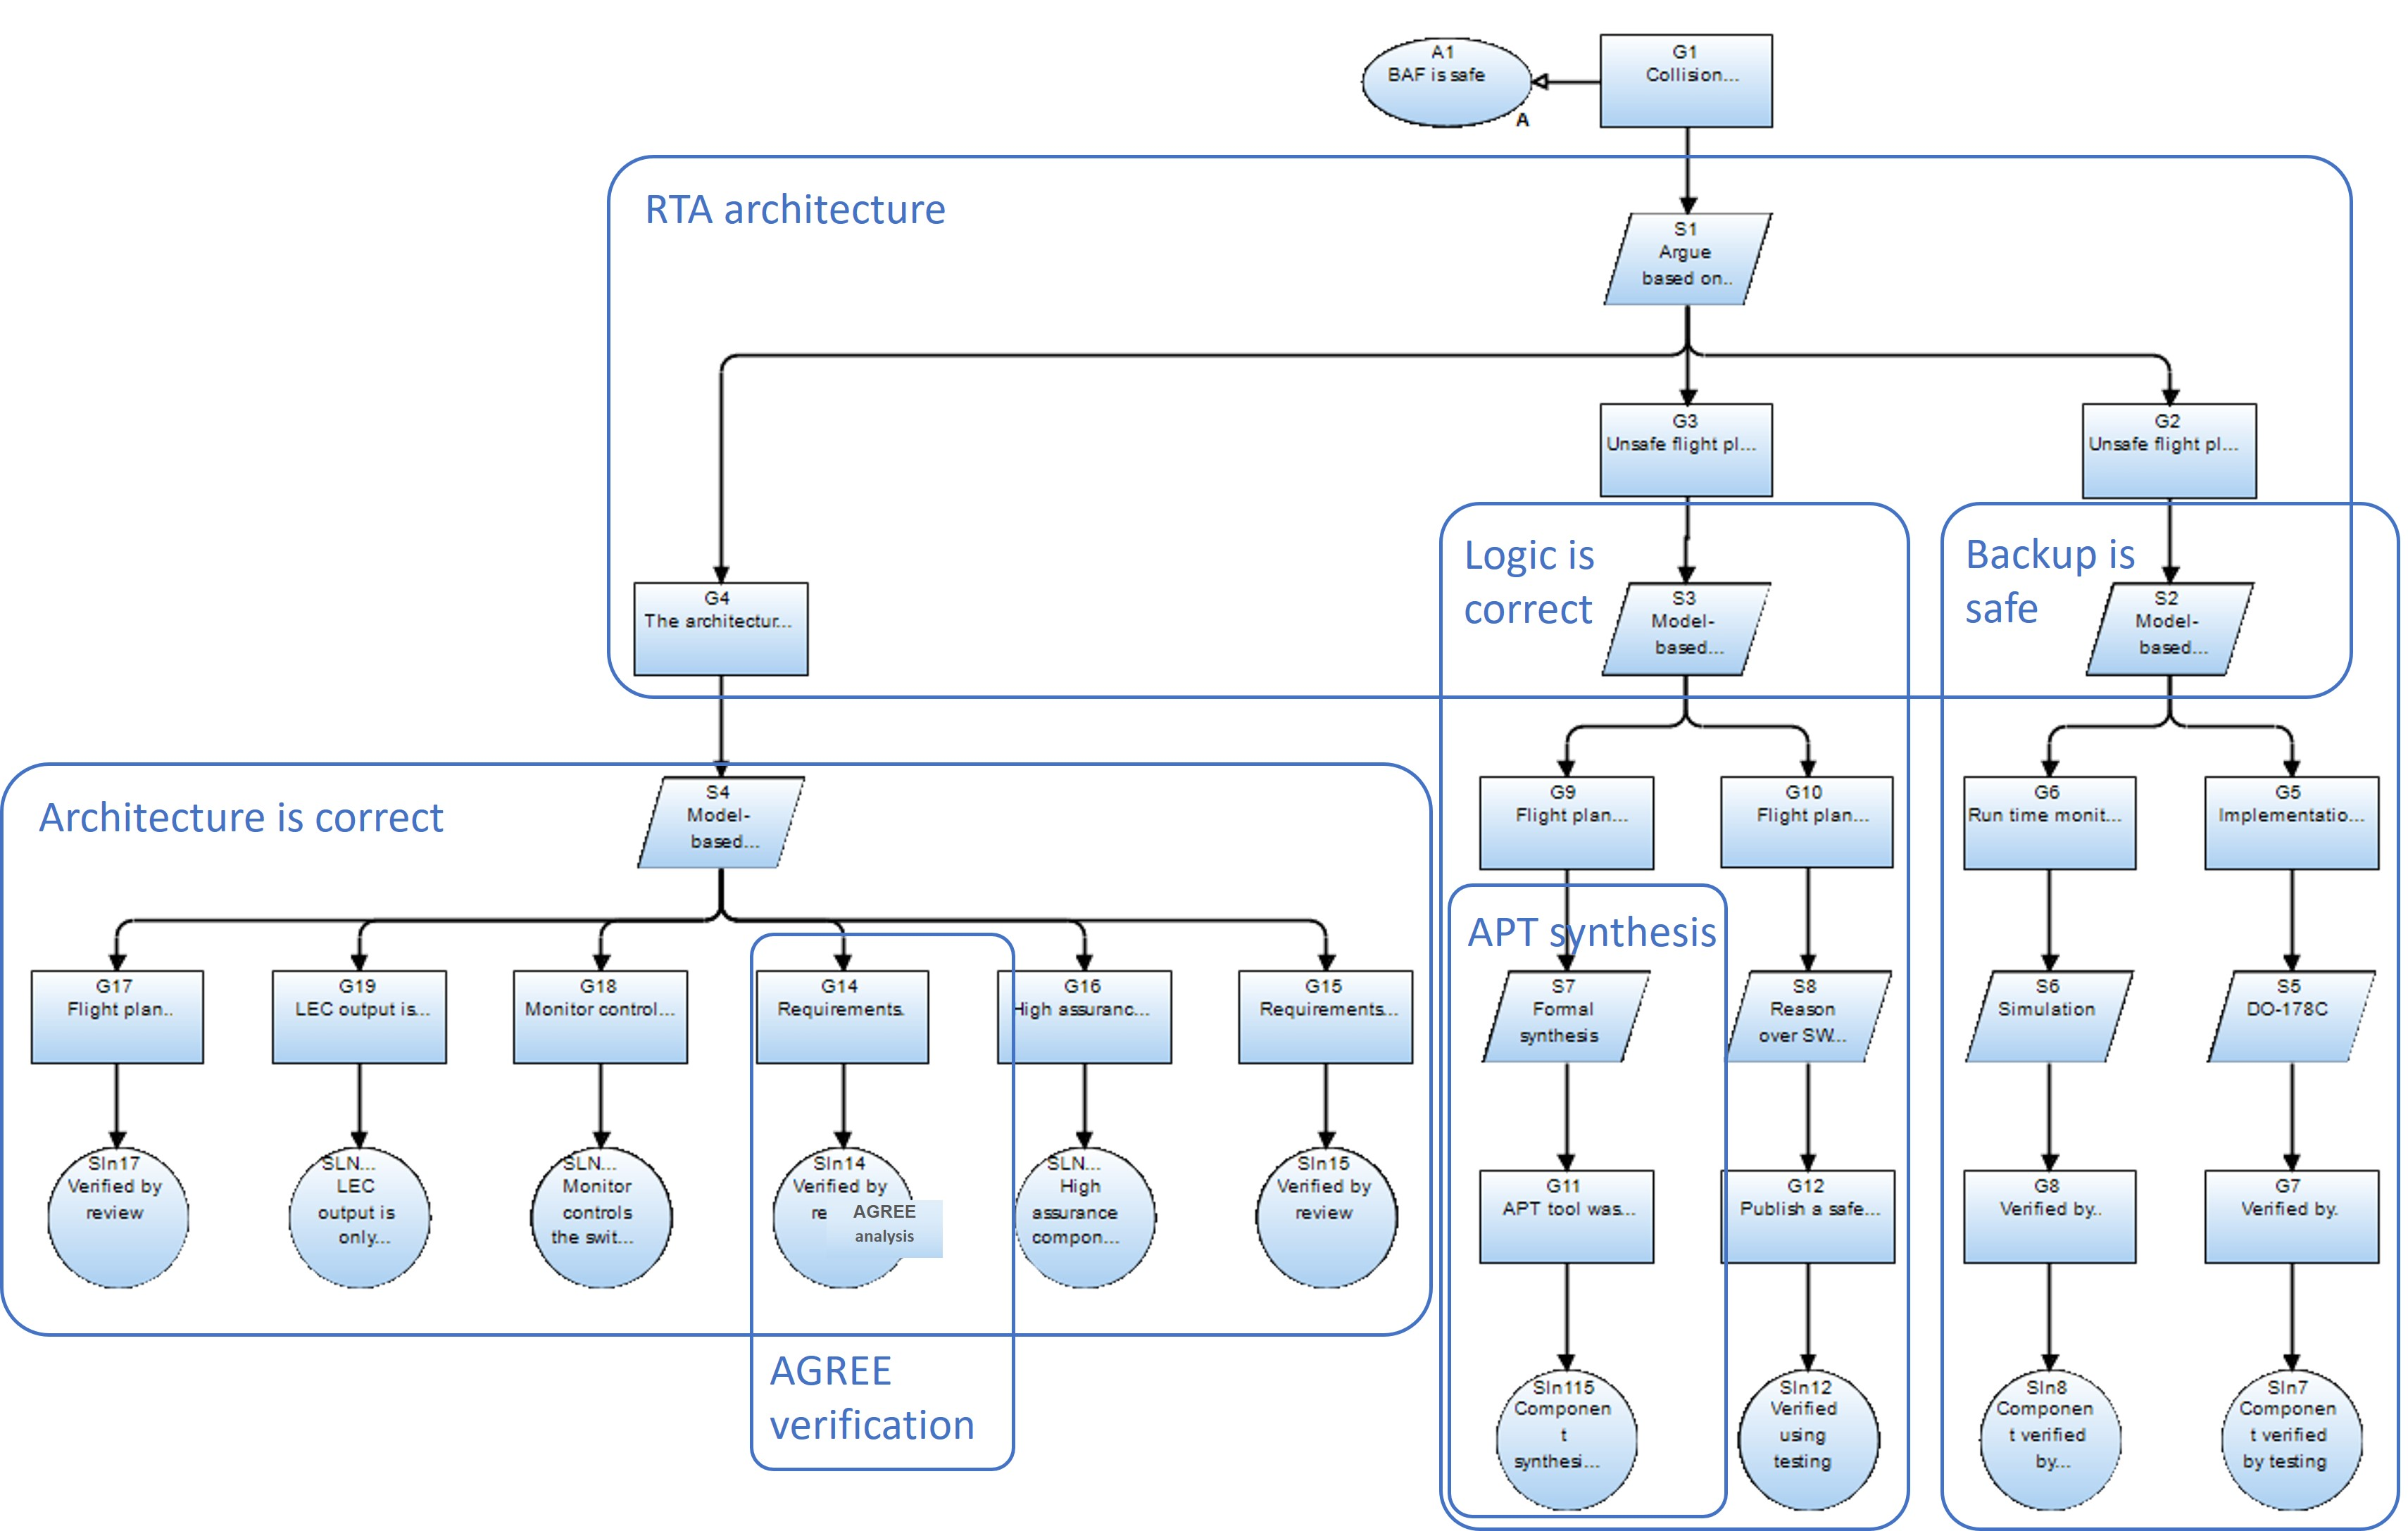
\includegraphics[width=\textwidth]{figures/rta-resolute.jpg}
	\caption{Assurance Argument for run-time assurance generated by Resolute}
	\label{fig:rta-resolute}
\end{figure*}
